% Chapter 1: Exploratory Data Analysis
\chapter{Exploratory Data Analysis}

\section{Introduction}
This project investigates forest fires in Algeria and Tunisia through a data mining approach. We integrate five datasets---fire records, land cover, climate, elevation, and soil---to understand fire occurrence factors. The objectives are:
\begin{enumerate}
    \item Collect and preprocess soil and climate data relevant to fire prediction.
    \item Apply supervised learning algorithms to predict fire occurrence.
    \item Use unsupervised learning (clustering) to identify natural groupings and high-risk areas.
    \item Evaluate model performance using standard metrics.
    \item Provide interpretable insights on fire risk zones.
\end{enumerate}

The repository structure and file descriptions are provided in Appendix~\ref{app:structure}.

\section{Fire Dataset}
The fire dataset is sourced from NASA's FIRMS (Fire Information for Resource Management System), providing active fire detections from VIIRS satellites.

\textbf{Key attributes} include: Latitude/Longitude (location), Brightness (fire intensity in Kelvin), FRP (Fire Radiative Power in MW), Confidence level, and Acquisition date/time.
\subsection{Descriptive statistics for fire datasets}

The following tables show descriptive statistics computed from the raw fire records for Algeria and Tunisia (numeric columns only).

\begin{table}[H]
    \centering
    \caption{Descriptive statistics — Algeria}
    \label{tab:desc_algeria}
    \resizebox{\textwidth}{!}{%
    \begin{tabular}{lrrrrrrrrr}
    \hline
    & latitude & longitude & bright\_ti4 & scan & track & acq\_time & bright\_ti5 & frp & type\\
    \hline
    count & 87446.000000 & 87446.000000 & 87446.000000 & 87446.000000 & 87446.000000 & 87446.000000 & 87446.000000 & 87446.000000 & 87446.000000\\
    mean  & 31.398370 & 6.174013 & 321.170189 & 0.476433 & 0.516127 & 379.367941 & 291.711062 & 3.454114 & 1.703863\\
    std   & 2.642515 & 2.563073 & 18.189028 & 0.101948 & 0.126665 & 479.842612 & 11.715804 & 5.018793 & 0.723168\\
    min   & 19.603230 & -8.118050 & 240.170000 & 0.320000 & 0.360000 & 0.000000 & 244.790000 & 0.060000 & 0.000000\\
    25%   & 28.735780 & 5.585470 & 305.500000 & 0.400000 & 0.400000 & 59.000000 & 282.860000 & 1.160000 & 2.000000\\
    50%   & 31.403925 & 6.475440 & 316.820000 & 0.450000 & 0.500000 & 141.000000 & 290.785000 & 2.080000 & 2.000000\\
    75%   & 32.515890 & 7.906365 & 337.420000 & 0.540000 & 0.620000 & 232.000000 & 298.100000 & 3.940000 & 2.000000\\
    max   & 37.022990 & 10.993650 & 367.000000 & 0.800000 & 0.780000 & 1410.000000 & 350.350000 & 251.890000 & 3.000000\\
    \hline
    \end{tabular}%
    }
\end{table}

\begin{table}[H]
    \centering
    \caption{Descriptive statistics — Tunisia}
    \label{tab:desc_tunisia}
    \resizebox{\textwidth}{!}{%
    \begin{tabular}{lrrrrrrrrr}
    \hline
    & latitude & longitude & bright\_ti4 & scan & track & acq\_time & bright\_ti5 & frp & type\\
    \hline
    count & 2804.000000 & 2804.000000 & 2804.000000 & 2804.000000 & 2804.000000 & 2804.000000 & 2804.000000 & 2804.000000 & 2804.000000\\
    mean  & 33.921434 & 9.586373 & 318.646933 & 0.462208 & 0.494215 & 410.385164 & 292.194807 & 3.250125 & 1.287803\\
    std   & 2.216090 & 0.615147 & 18.551266 & 0.088829 & 0.119610 & 506.203390 & 11.196871 & 9.601906 & 0.959535\\
    min   & 30.987250 & 8.163090 & 295.000000 & 0.320000 & 0.360000 & 1.000000 & 253.910000 & 0.110000 & 0.000000\\
    25%   & 31.649180 & 9.170558 & 302.560000 & 0.397500 & 0.380000 & 55.000000 & 283.877500 & 0.840000 & 0.000000\\
    50%   & 33.531755 & 9.490375 & 311.930000 & 0.440000 & 0.460000 & 129.000000 & 290.890000 & 1.490000 & 2.000000\\
    75%   & 36.501883 & 10.027000 & 336.372500 & 0.510000 & 0.590000 & 1134.250000 & 297.955000 & 3.452500 & 2.000000\\
    max   & 37.323460 & 11.110350 & 367.000000 & 0.800000 & 0.780000 & 1333.000000 & 355.420000 & 191.940000 & 3.000000\\
    \hline
    \end{tabular>%
    }
\end{table}

\subsection{Spatial Distribution}
Figure~\ref{fig:fire_spatial_algeria} and Figure~\ref{fig:fire_spatial_tunisia} display the geographic distribution of fire detections overlaid on country boundaries.

\begin{figure}[H]
    \centering
    \begin{minipage}{0.48\textwidth}
        \centering
        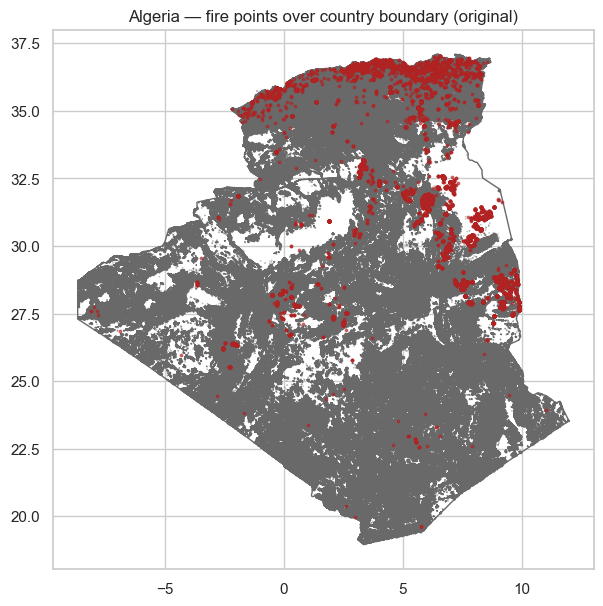
\includegraphics[width=\textwidth]{ressources/chapter1/fire_algeria.png}
        \caption{Fire detections in Algeria}
        \label{fig:fire_spatial_algeria}
    \end{minipage}
    \hfill
    \begin{minipage}{0.48\textwidth}
        \centering
        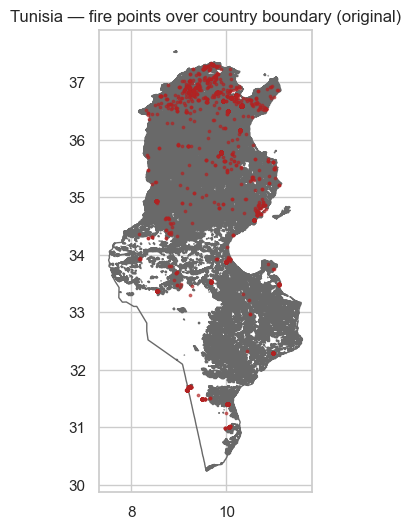
\includegraphics[width=\textwidth]{ressources/chapter1/fire_tunisia.png}
        \caption{Fire detections in Tunisia}
        \label{fig:fire_spatial_tunisia}
    \end{minipage}
\end{figure}

\textbf{Spatial insights:} Fires concentrate in northern coastal regions with Mediterranean vegetation, mountainous forested areas (Atlas Mountains), and transition zones between Mediterranean and semi-arid climates. Algeria exhibits significantly more fire detections (87,446) compared to Tunisia (2,804), reflecting both country size and vegetation density differences.

\subsection{Univariate Analysis}
Figure~\ref{fig:fire_univariate} presents histograms and boxplots for key fire attributes, comparing distributions between Algeria and Tunisia.

\begin{figure}[H]
    \centering
    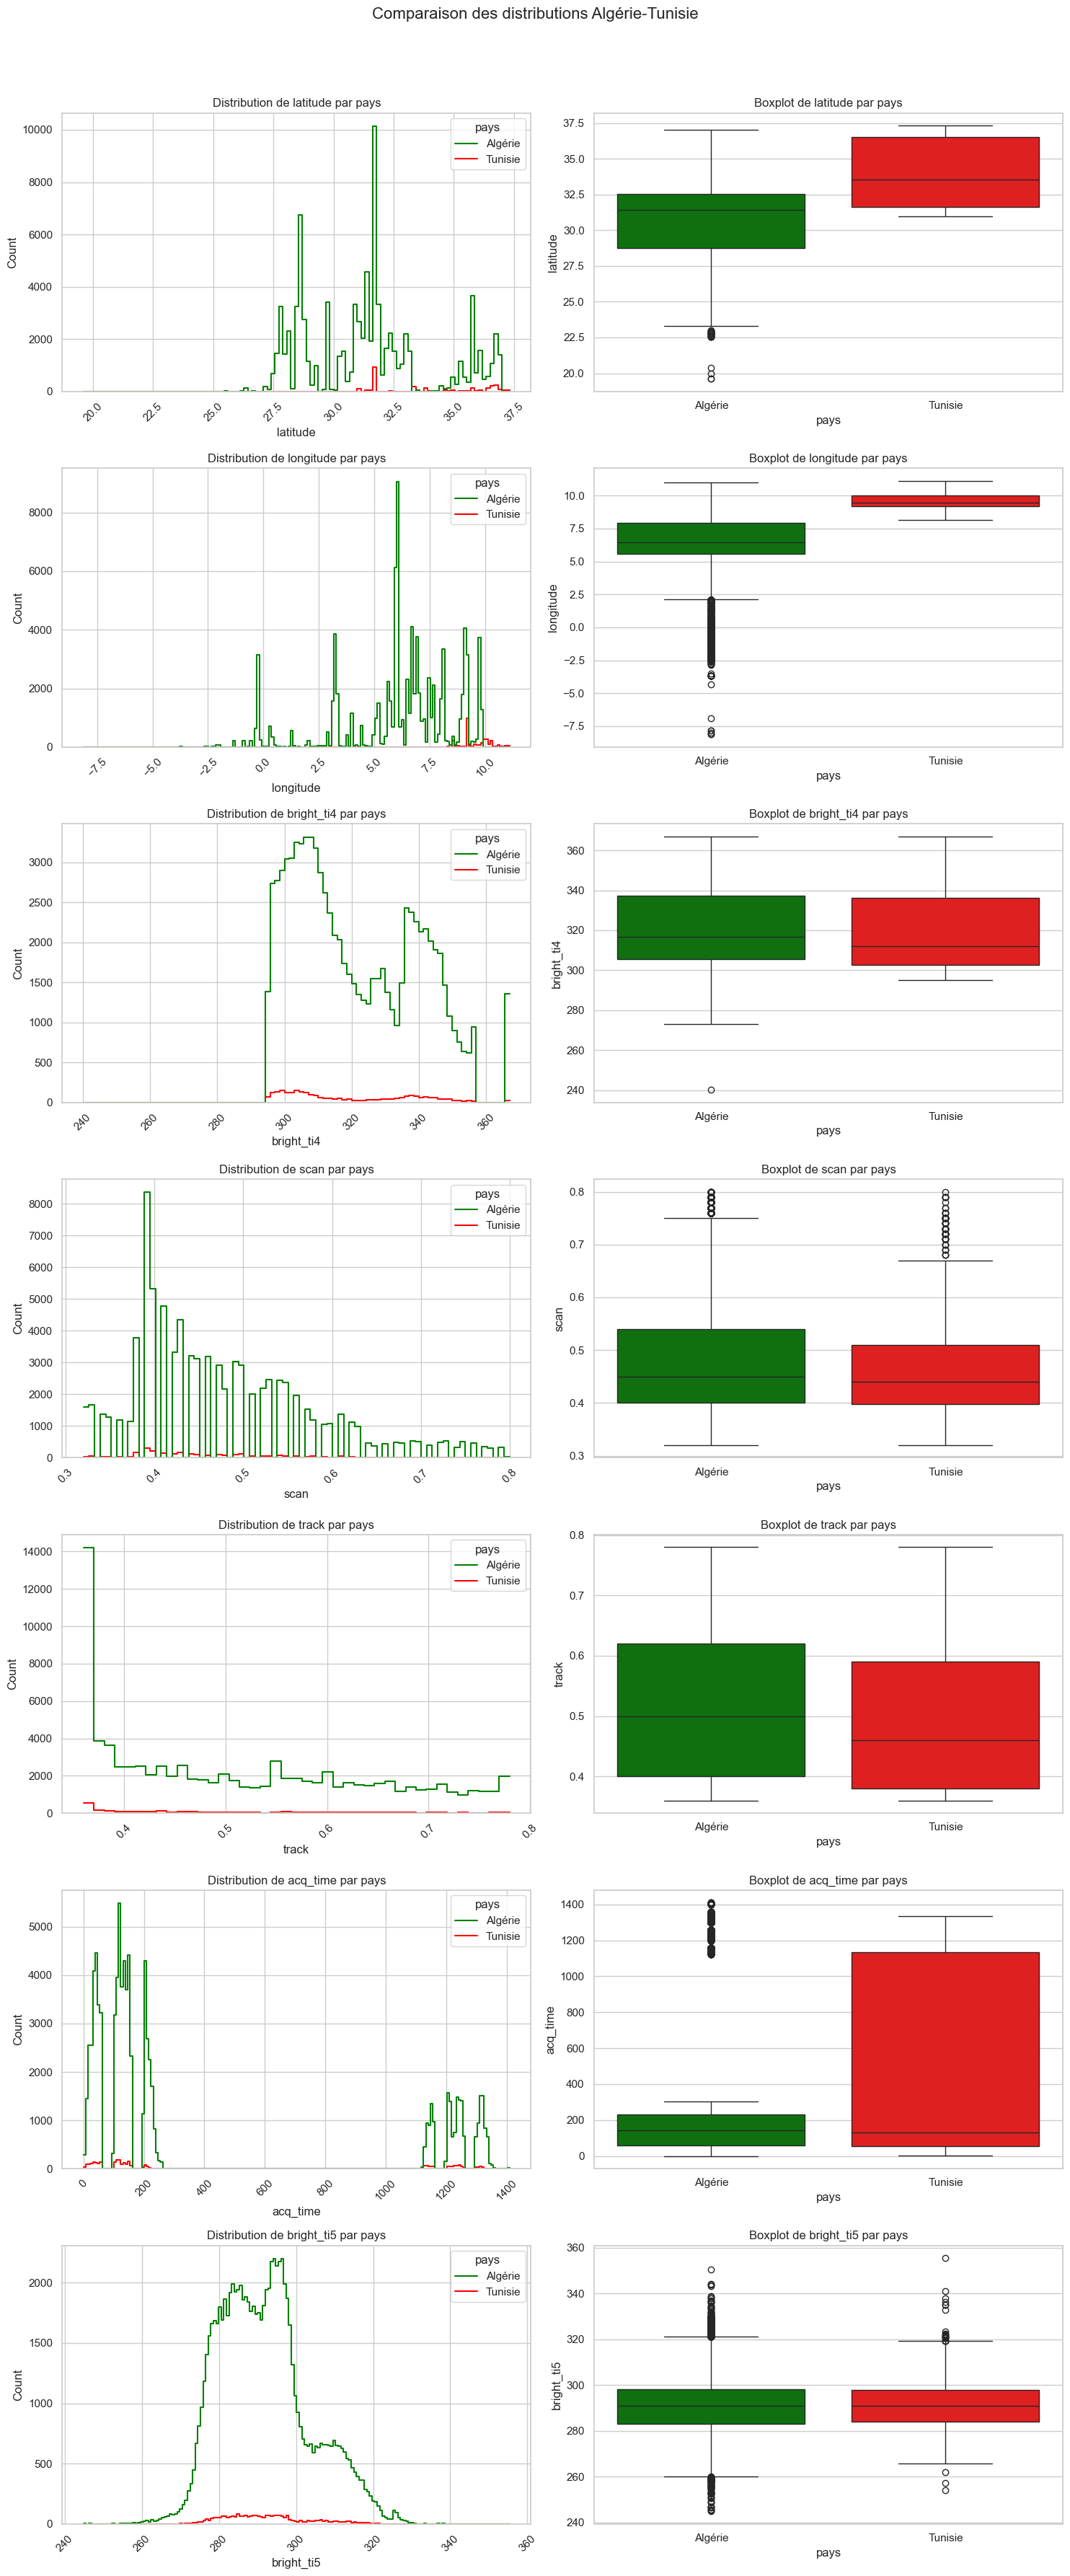
\includegraphics[width=0.85\textwidth]{ressources/chapter1/fire_univariate.png}
    \caption{Distribution of fire attributes (brightness, FRP, scan, track) by country}
    \label{fig:fire_univariate}
\end{figure}

\textbf{Fire column note:} The `type` column encodes detection classification (sensor/processing category) and is useful for filtering and assessing detection quality when analyzing fire records. In our data the observed values include `0`, `1`, and `2`. We treat `0` as the primary active fire detection class and retain these records for analysis. Records with `type=2` are considered non-standard or lower-confidence detections (more likely to contain false positives), so we removed `type=2` from the analysis to focus on higher-confidence events representative of forest fires.

\begin{figure}[H]
    \centering
    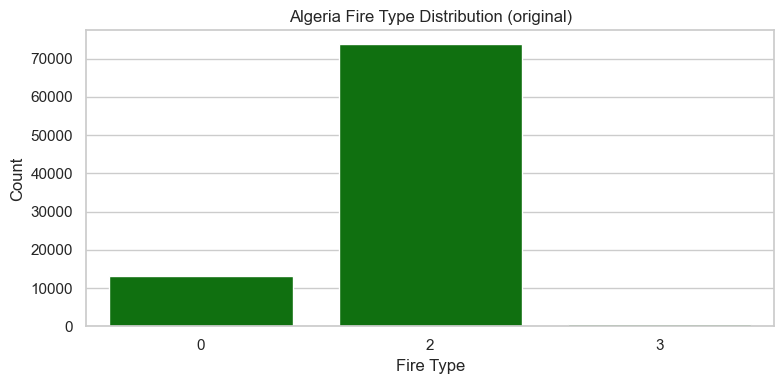
\includegraphics[width=0.5\textwidth]{ressources/chapter1/fire_type_distribution.png}
    \caption{Fire type distribution}
    \label{fig:fire_type_dist}
\end{figure}

\textbf{Univariate insights:} Both countries show similar brightness temperature distributions (mean $\approx$ 320~K), indicating comparable fire intensities. Fire Radiative Power (FRP) is right-skewed with most fires being low-intensity events. Outliers in FRP represent extreme fire events requiring special attention in modeling.

\subsection{Bivariate Analysis}
Figure~\ref{fig:fire_qq_bright} and Figure~\ref{fig:fire_qq_frp} present Q-Q plots comparing the distributions of key fire attributes between Algeria and Tunisia.

\begin{figure}[H]
    \centering
    \begin{minipage}{0.48\textwidth}
        \centering
        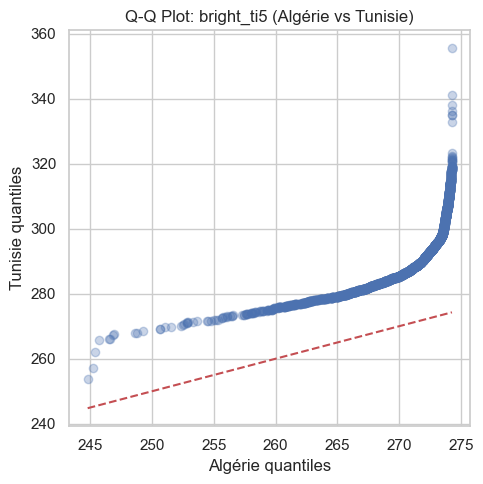
\includegraphics[width=\textwidth]{ressources/chapter1/fire_qq_bright.png}
        \caption{Q-Q plot: Brightness (Algeria vs Tunisia)}
        \label{fig:fire_qq_bright}
    \end{minipage}
    \hfill
    \begin{minipage}{0.48\textwidth}
        \centering
        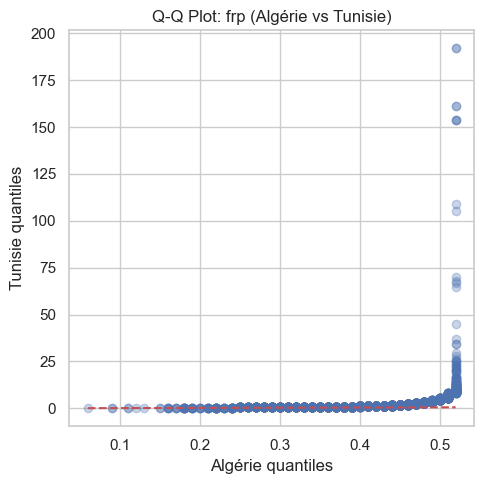
\includegraphics[width=\textwidth]{ressources/chapter1/fire_qq_frp.png}
        \caption{Q-Q plot: FRP (Algeria vs Tunisia)}
        \label{fig:fire_qq_frp}
    \end{minipage}
\end{figure}

\textbf{Q-Q insights:} The Q-Q plots reveal that brightness distributions are similar between countries (points close to the diagonal), while FRP shows deviations indicating different intensity profiles.

Figure~\ref{fig:fire_heatmap} displays the correlation matrix between fire attributes.

\begin{figure}[H]
    \centering
    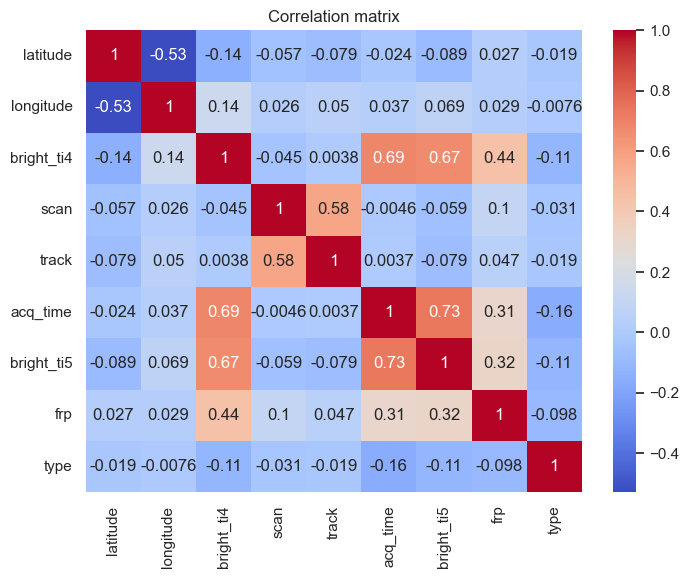
\includegraphics[width=0.85\textwidth]{ressources/chapter1/fire_heatmap.png}
    \caption{Correlation heatmap of fire variables}
    \label{fig:fire_heatmap}
\end{figure}

\textbf{Correlation insights:} Strong positive correlation exists between brightness temperatures (bright\_ti4 and bright\_ti5). FRP correlates moderately with brightness, confirming that hotter fires release more energy.

Figure~\ref{fig:fire_scatter} shows pairwise scatter plots between selected fire attributes.

\begin{figure}[H]
    \centering
    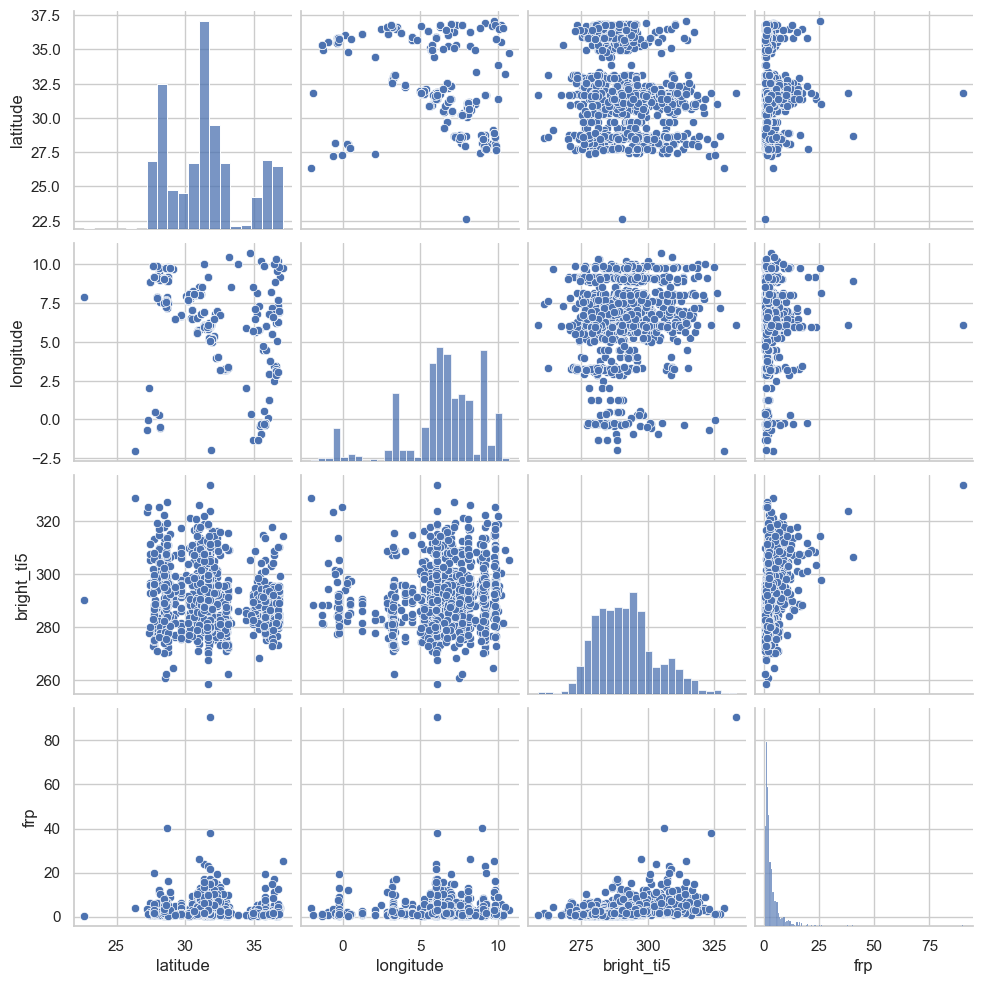
\includegraphics[width=0.85\textwidth]{ressources/chapter1/fire_scatter.png}
    \caption{Pairwise scatter plots of fire variables}
    \label{fig:fire_scatter}
\end{figure}

\textbf{Scatter insights:} Geographic coordinates (latitude, longitude) show weak correlation with intensity metrics, suggesting fire severity is independent of location. The scatter plots also reveal clustering patterns in fire occurrence.

\subsection{Temporal Analysis}
Figure~\ref{fig:fire_daily} and Figure~\ref{fig:fire_weekly} show daily and weekly fire counts throughout the year, highlighting short-term variability and smoothed seasonal trends respectively.

\begin{figure}[H]
    \centering
    \begin{minipage}{0.48\textwidth}
        \centering
        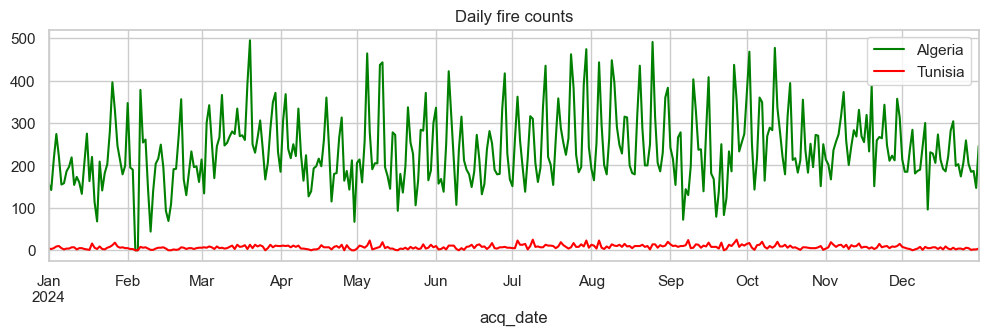
\includegraphics[width=\textwidth]{ressources/chapter1/fire_daily_counts.png}
        \caption{Daily fire counts}
        \label{fig:fire_daily}
    \end{minipage}
    \hfill
    \begin{minipage}{0.48\textwidth}
        \centering
        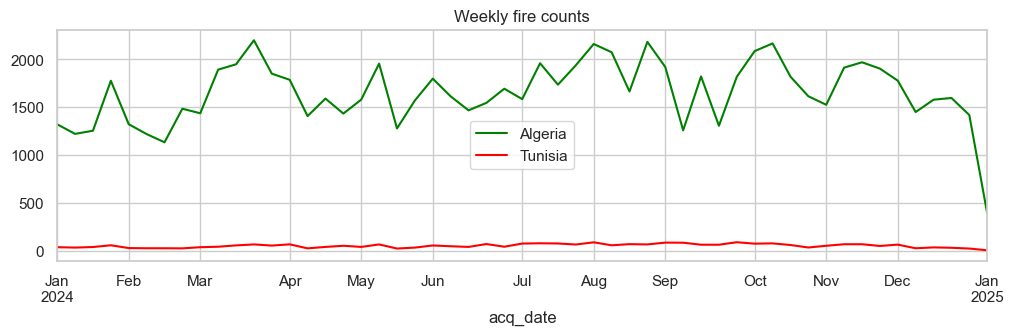
\includegraphics[width=\textwidth]{ressources/chapter1/fire_weekly_counts.png}
        \caption{Weekly fire counts}
        \label{fig:fire_weekly}
    \end{minipage}
\end{figure}

\textbf{Temporal insights:} Daily counts show short-term variability and potential sequencing of events, while weekly aggregations smooth noise and clearly reveal the seasonal peak in summer months (June--September), with August typically the busiest month.

\section{Land Cover Dataset}
Land cover data from the FAO Global Land Cover Share database classifies surface types including forests, shrublands, grasslands, croplands, urban areas, bare land, and water bodies.

\textbf{Key finding:} Forests and shrublands show the highest fire incidence due to fuel availability. Bare lands and urban areas have minimal fire activity. This relationship guided our decision to include land cover as a feature in modeling.

\begin{figure}[H]
    \centering
    \includegraphics[width=0.85\textwidth]{ressources/chapter1/landcover.png}
    \caption{Land cover classification and fire occurrence by vegetation type}
    \label{fig:landcover}
\end{figure}

\section{Climate Dataset}
Climate data comes from CHIRPS (precipitation) and TerraClimate (temperature) with monthly resolution at approximately 4~km spatial resolution.

\textbf{Variables:} Precipitation (mm/month), Maximum temperature (°C), Minimum temperature (°C).

\textbf{Climate-fire relationship:} The Mediterranean climate of the study region shows strong correlation with fire patterns:
\begin{itemize}
    \item \textbf{Temperature:} Positive correlation with fire occurrence
    \item \textbf{Precipitation:} Negative correlation---drought conditions elevate risk
    \item \textbf{Decision:} We derived a drought index combining temperature and precipitation effects
\end{itemize}

\begin{figure}[H]
    \centering
    \includegraphics[width=0.85\textwidth]{ressources/chapter1/climate.png}
    \caption{Seasonal climate patterns and correlation with fire occurrence}
    \label{fig:climate}
\end{figure}

\section{Elevation Dataset}
Elevation data from GMTED2010 provides a Digital Elevation Model at 15 arc-second resolution (approximately 500~m).

\textbf{Topographic analysis:}
\begin{itemize}
    \item \textbf{Slope:} Steeper slopes promote faster fire spread (preheating of upslope fuels)
    \item \textbf{Aspect:} South-facing slopes are drier due to solar radiation
    \item \textbf{Decision:} We derived terrain complexity and coastal proximity as additional features
\end{itemize}

\begin{figure}[H]
    \centering
    \includegraphics[width=0.85\textwidth]{ressources/chapter1/elevation.png}
    \caption{Digital elevation model and derived topographic features}
    \label{fig:elevation}
\end{figure}

\section{Soil Dataset}
Soil data from the Harmonized World Soil Database v2.0 (HWSD2) provides properties including organic carbon, nitrogen, pH, and texture fractions (sand, clay, silt).

\textbf{Soil-fire relationship:}
\begin{itemize}
    \item \textbf{Organic carbon:} Higher content supports denser vegetation, increasing fuel loads
    \item \textbf{Soil texture:} Sandy soils drain faster, leading to drier conditions
    \item \textbf{Decision:} We included soil properties as secondary predictors
\end{itemize}

\begin{figure}[H]
    \centering
    \includegraphics[width=0.85\textwidth]{ressources/chapter1/soil.png}
    \caption{Soil classification and properties at fire locations}
    \label{fig:soil}
\end{figure}

\section{Summary}
The exploratory analysis reveals:
\begin{itemize}
    \item \textbf{Fire Dataset:} Strong seasonal patterns (summer peak) and spatial concentration in northern forested regions
    \item \textbf{Land Cover:} Forests and shrublands are most fire-prone
    \item \textbf{Climate:} Mediterranean patterns strongly influence fire occurrence
    \item \textbf{Elevation:} Topography affects fire behavior through slope and aspect
    \item \textbf{Soil:} Subsurface factors affect vegetation and moisture
\end{itemize}

These insights inform preprocessing and feature engineering decisions in subsequent chapters.
